\section*{\textbf{Resident North American birds range limits}}
We estimated the geographic range limits of the 96 resident North American birds used in our analyses that had geographic ranges in birdLife. Overall, species commonly have geographic range limits that represent the terrestrial boundaries of North America (Figure \ref{fig:rangelimits}), suggesting that range limits may often not represent niche limits. 

\begin{figure}[H]
\centering
\centerline{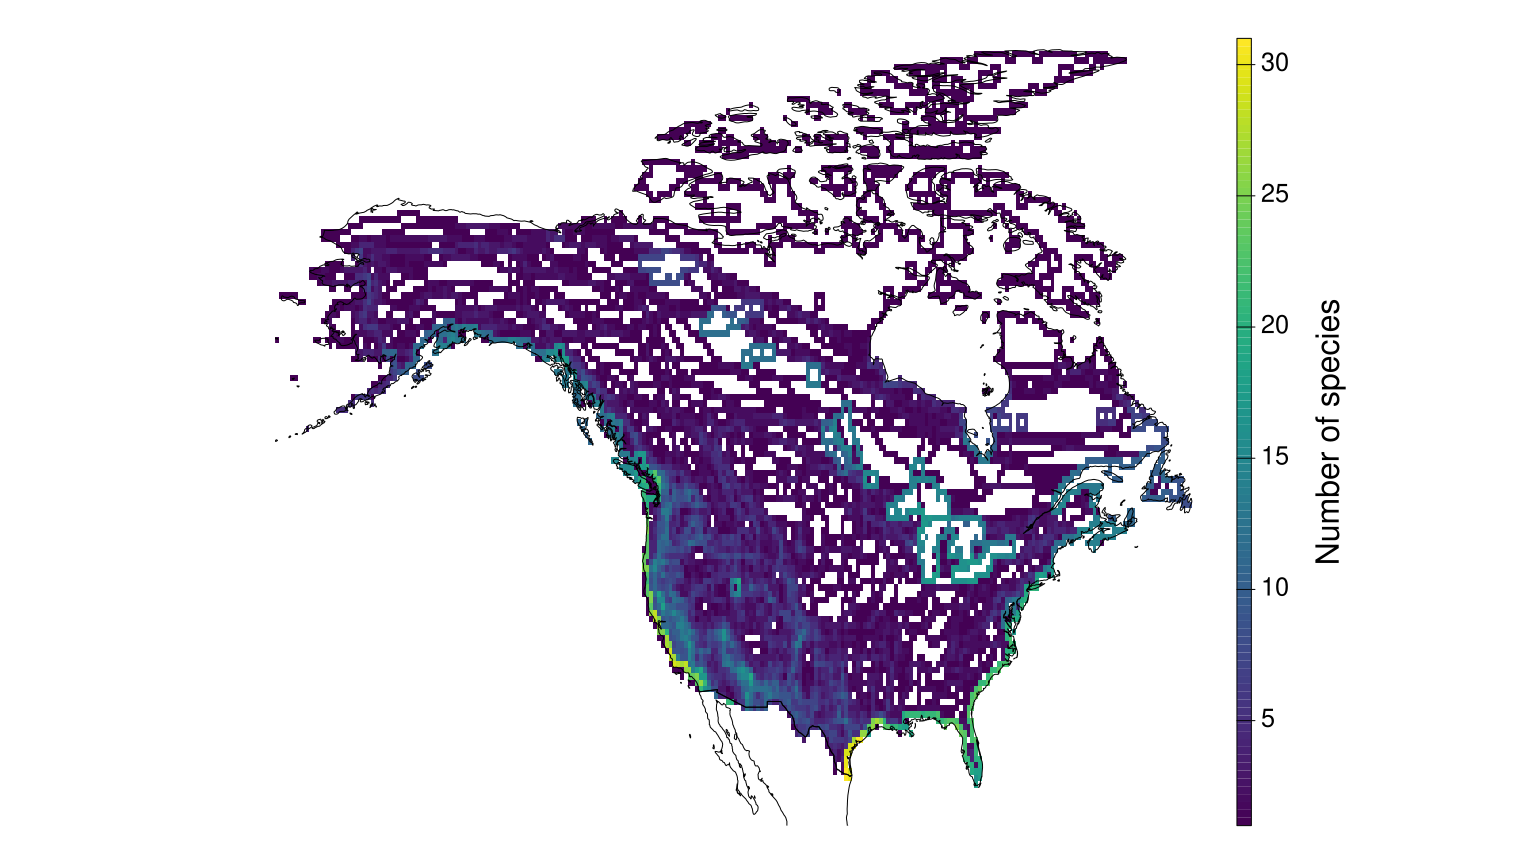
\includegraphics[width=1\textwidth]{FigRange/rangelimits.png}}
\caption[Geographic range limits]{Geographic range limits of 96 resident North American birds that have expert geographic ranges. Species more often have geographic range limits near the terrestrial borders of North America than within the continent, indicating that geographic ranges of several species may not be limited by their climatic niche. The colors represent the number of species that have geographic range edges in a given location.}  
\label{fig:rangelimits}
\end{figure}
\section*{\textbf{Sites sampled by the Breeding Bird Survey}}
The species considered in our study were observed in a total of 4803 routes that were sampled between 1997 and 2019 by the BBS. About 3051$\pm$127 routes were sampled annually and routes were sampled on average for 15$\pm$7 years (Figure \ref{fig:routes}). 
\begin{figure}[H]
\centering
\centerline{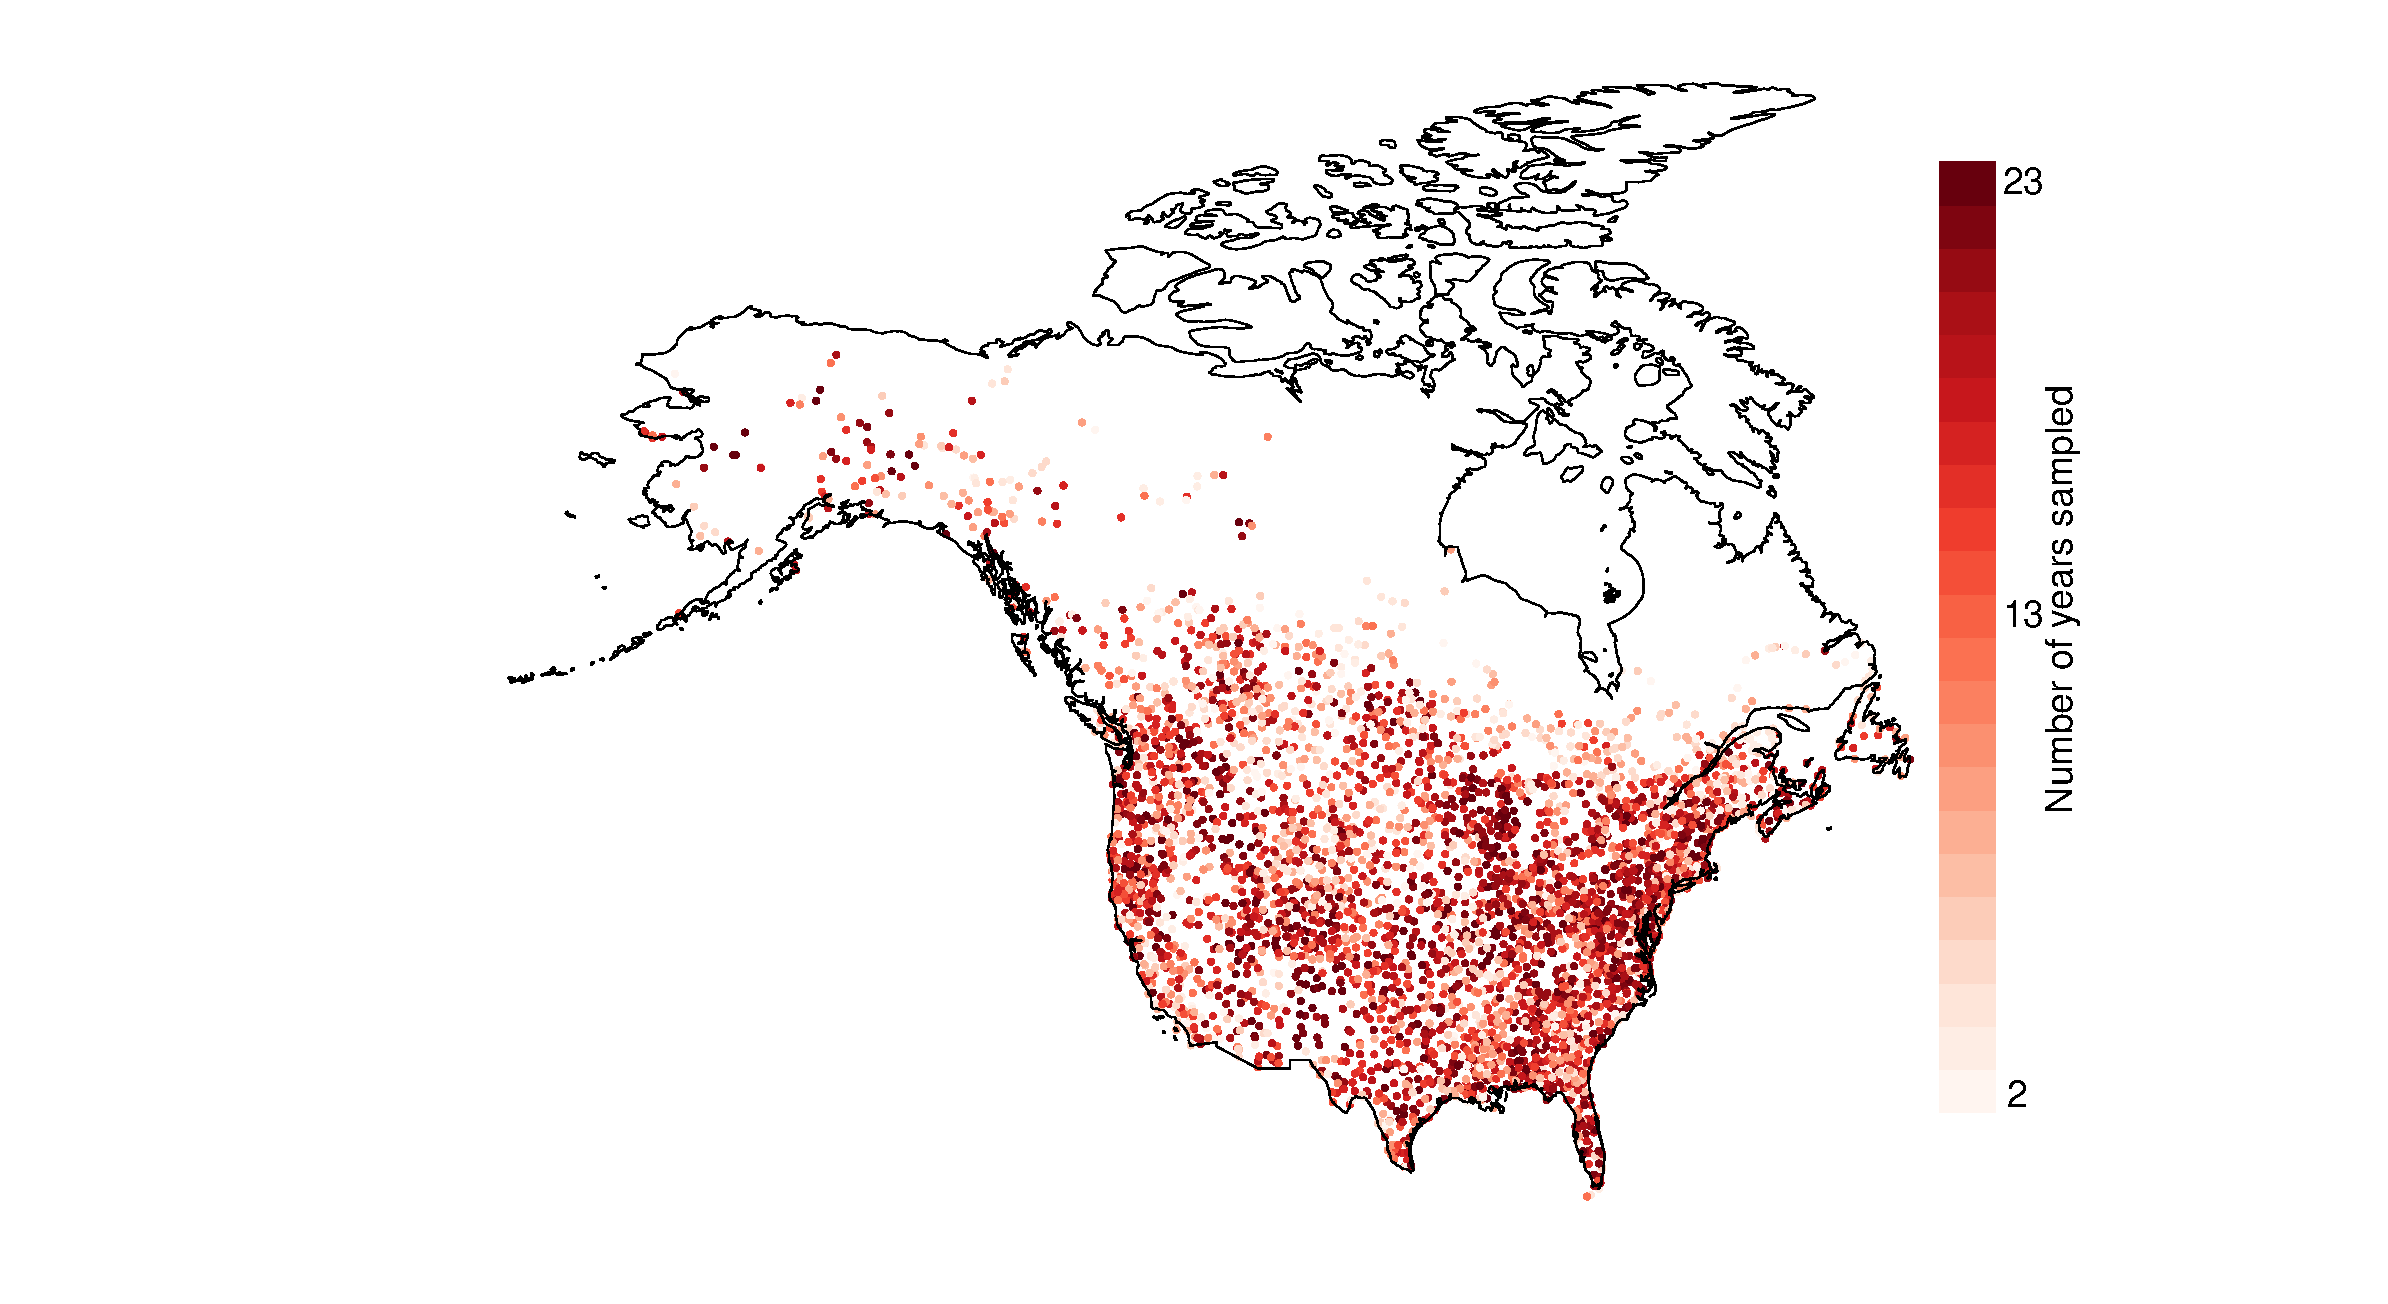
\includegraphics[width=1\textwidth]{FigRange/yearsampled}}
\caption[Routes sampled by the Breeding Bird Survey]{Routes sampled by BBS between 1997 and 2019 where the species used in our analyses occurred. Routes were well sampled during this time period, with an average of $\approx$ 3000 routes sampled yearly. Colors represent the number of years routes were sampled between 1997 and 2019.}  
\label{fig:routes}
\end{figure}
\section*{\textbf{Model diagnostics}}
Model diagnostics for the linear mixed models that we fit were done using the \texttt{performance} R package. We checked model convergence and singularity using the functions \textit{check$\_$convergence} and \textit{check$\_$singularity}. Heteroscedasticity was checked for using the function \textit{check$\_$heteroscedasticity}, which performs the Breusch-Paga test for heteroscedasticity. Overdispersion and underdispersion were checked using the function \textit{check$\_$overdispersion}. Additionally, visual checks were also performed for all models using the \textit{check$\_$model} function. All models that we fit successfully converged, were not singular, had homoscedastic error variance, and were not over or underdispersed. Visual checks also indicated that model assumptions were generally met (Figures \ref{fig:main_mod}-\ref{fig:comp_mod}), suggesting that our results are robust. 

\begin{figure}[H]
\centering
\centerline{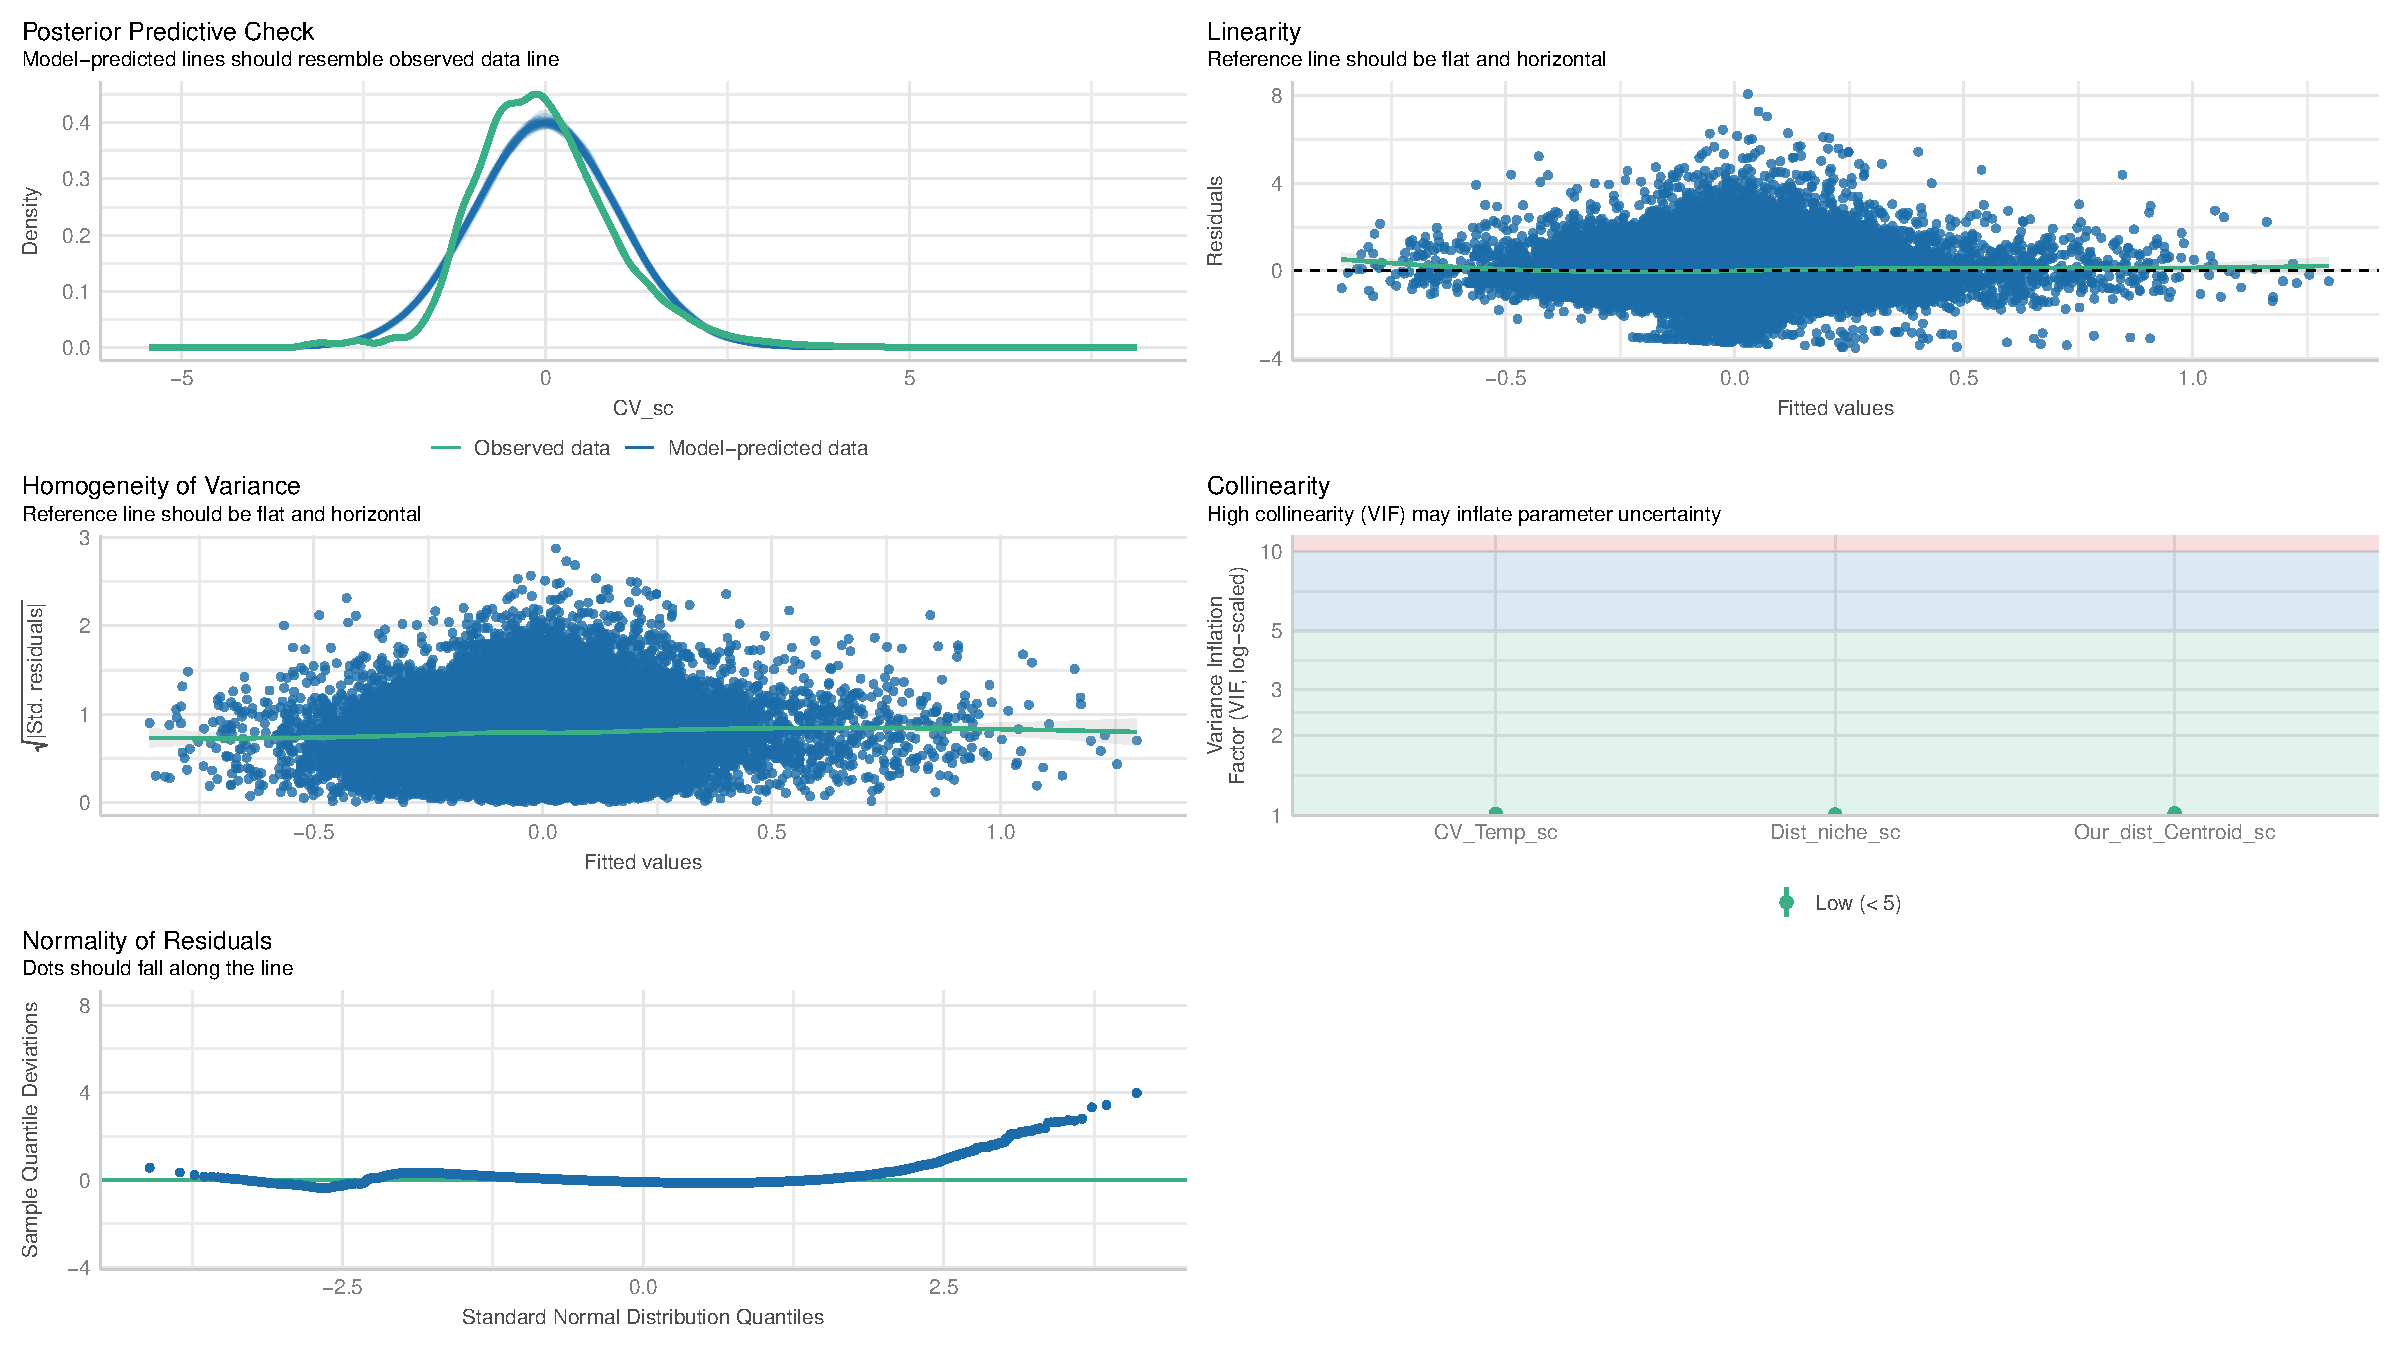
\includegraphics[width=1\textwidth]{FigRange/mod_main}}
\caption[Main model diagnostics]{Visual model diagnostics for the model used to report the results in the main text (Table \ref{tab:lmm_main}). Overall, the gaussian family fits well to the response variable that we used in the models (CV$\_$sc; scaled population variability), the linearity assumption is met, variance is homogeneous, there is not correlation between the predictor variables (i.e., variance inflation factor (VIF) < 5), and the residuals are normally distributed.}  
\label{fig:main_mod}
\end{figure}

\begin{figure}[H]
\centering
\centerline{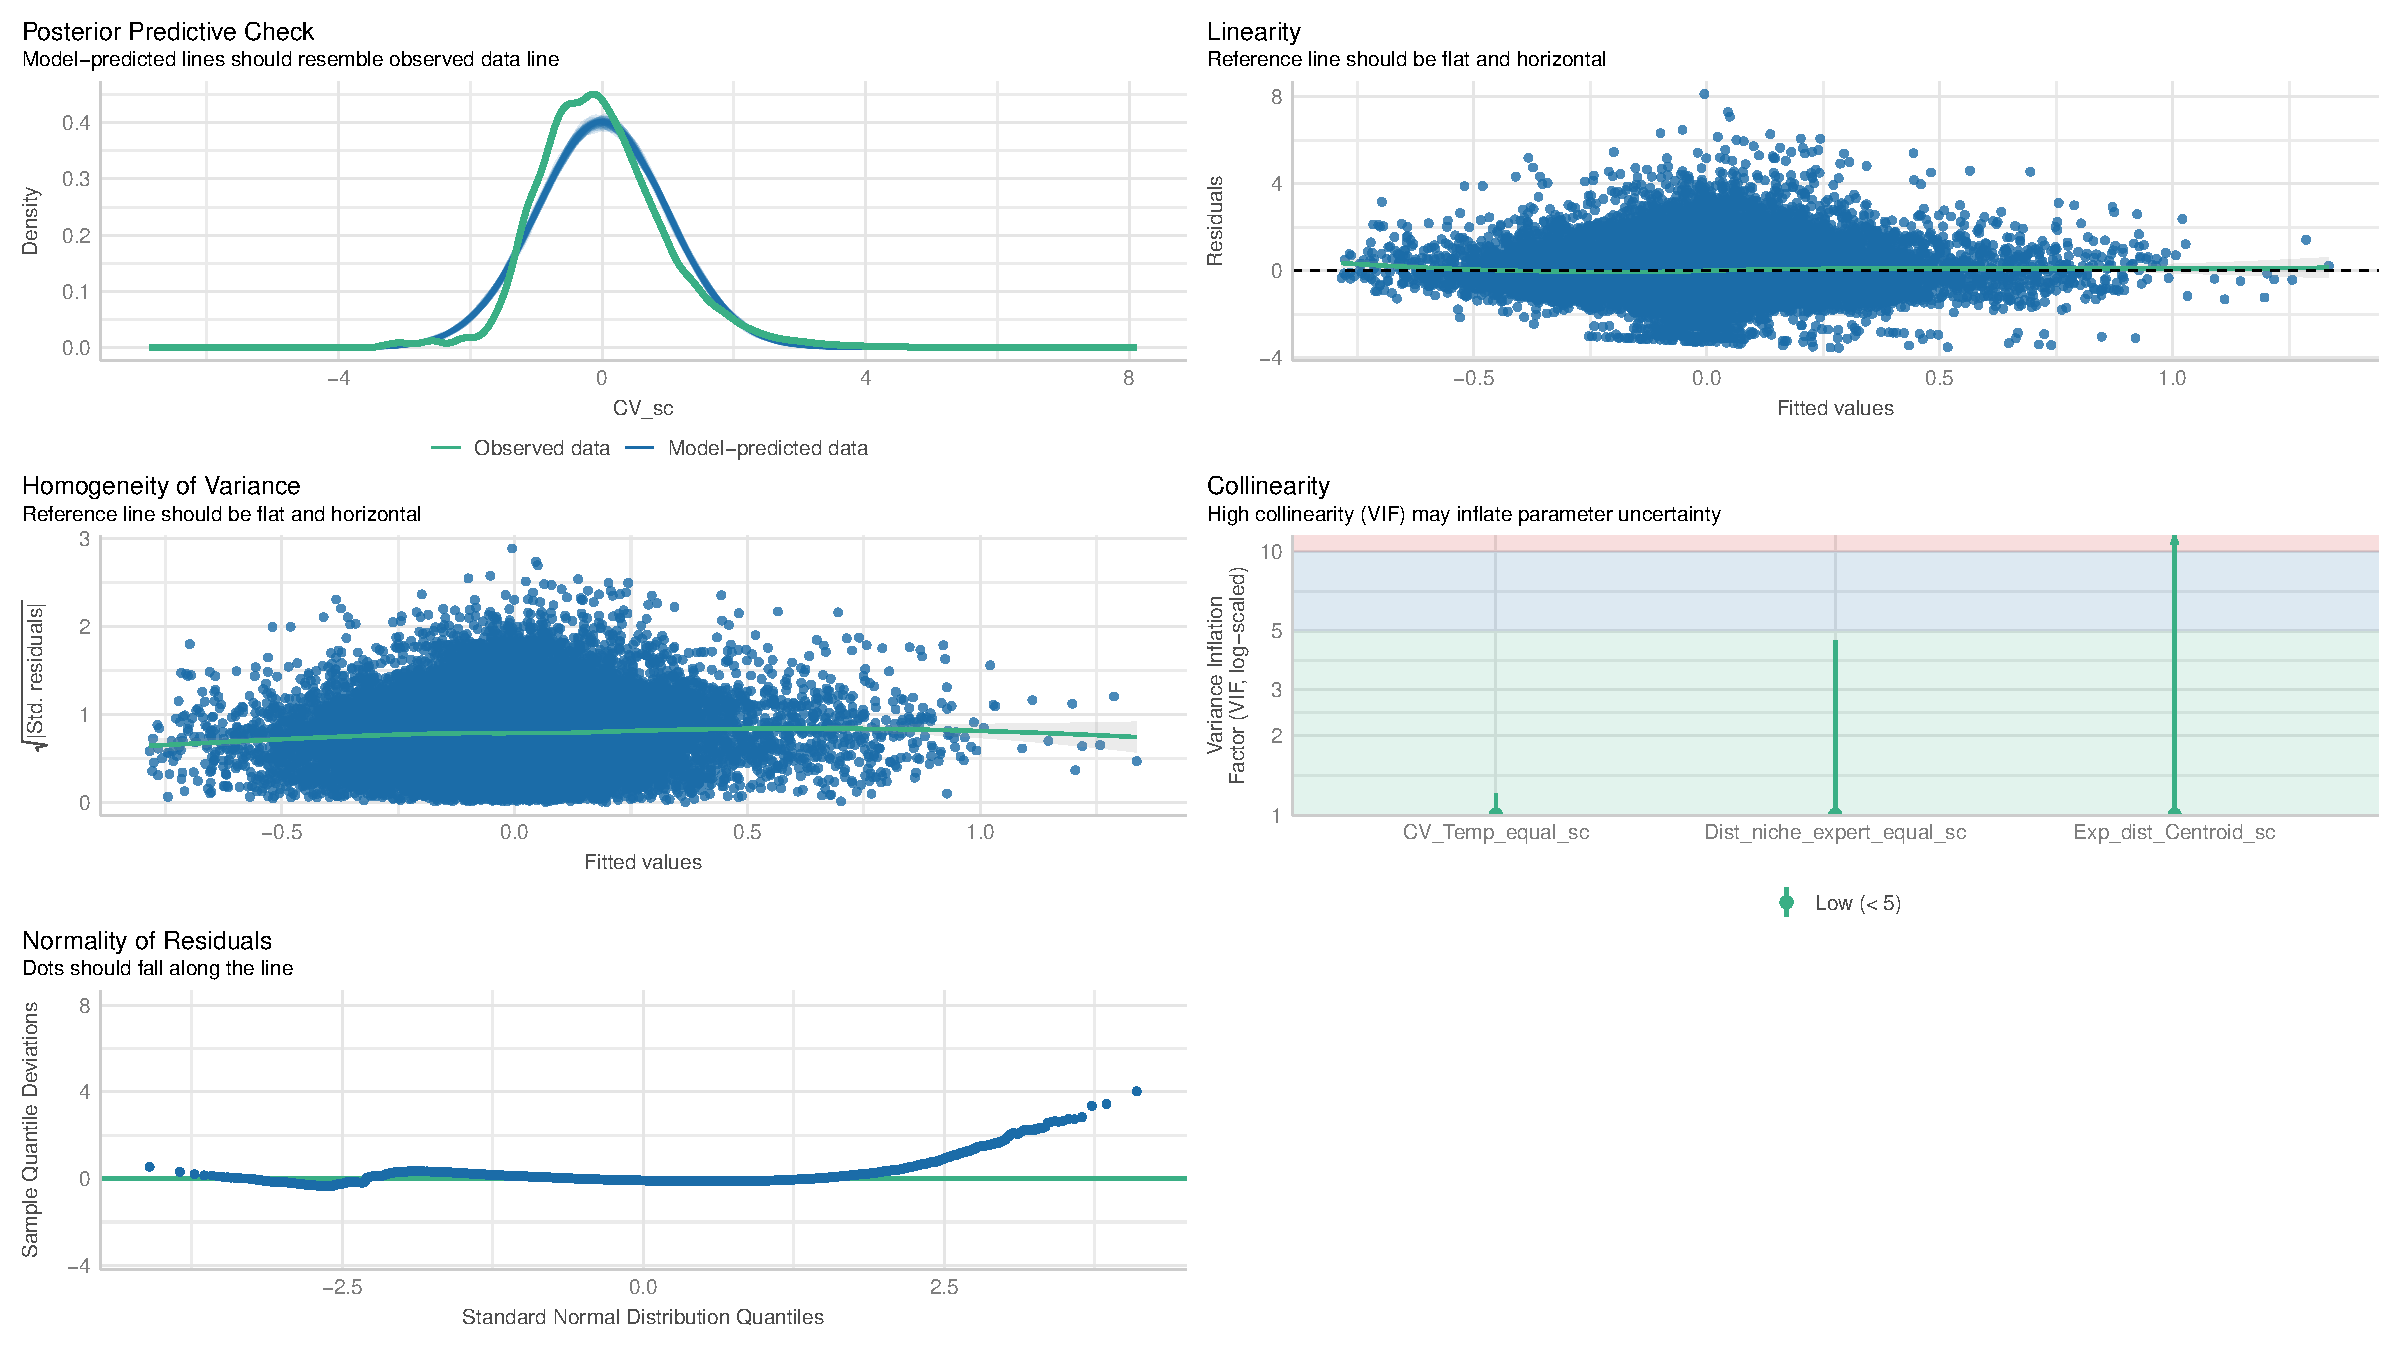
\includegraphics[width=1\textwidth]{FigRange/mod_exp}}
\caption[Expert model diagnostics]{Visual model diagnostics for the model that estimated distance to geographic range center and climatic niche position from expert ranges, and that used temperature variability data aggregated from Behrmann equal area projection, as predictors (Table \ref{tab:lmm_exp}). Overall, the gaussian family fits well to the response variable that we used in the models (CV$\_$sc; scaled population variability), the linearity assumption is met, variance is homogeneous, and there is relatively low correlation between the predictor variables (i.e., variance inflation factor (VIF) often < 5), and the residuals are normally distributed.}  
\label{fig:exp_mod}
\end{figure}

\begin{figure}[H]
\centering
\centerline{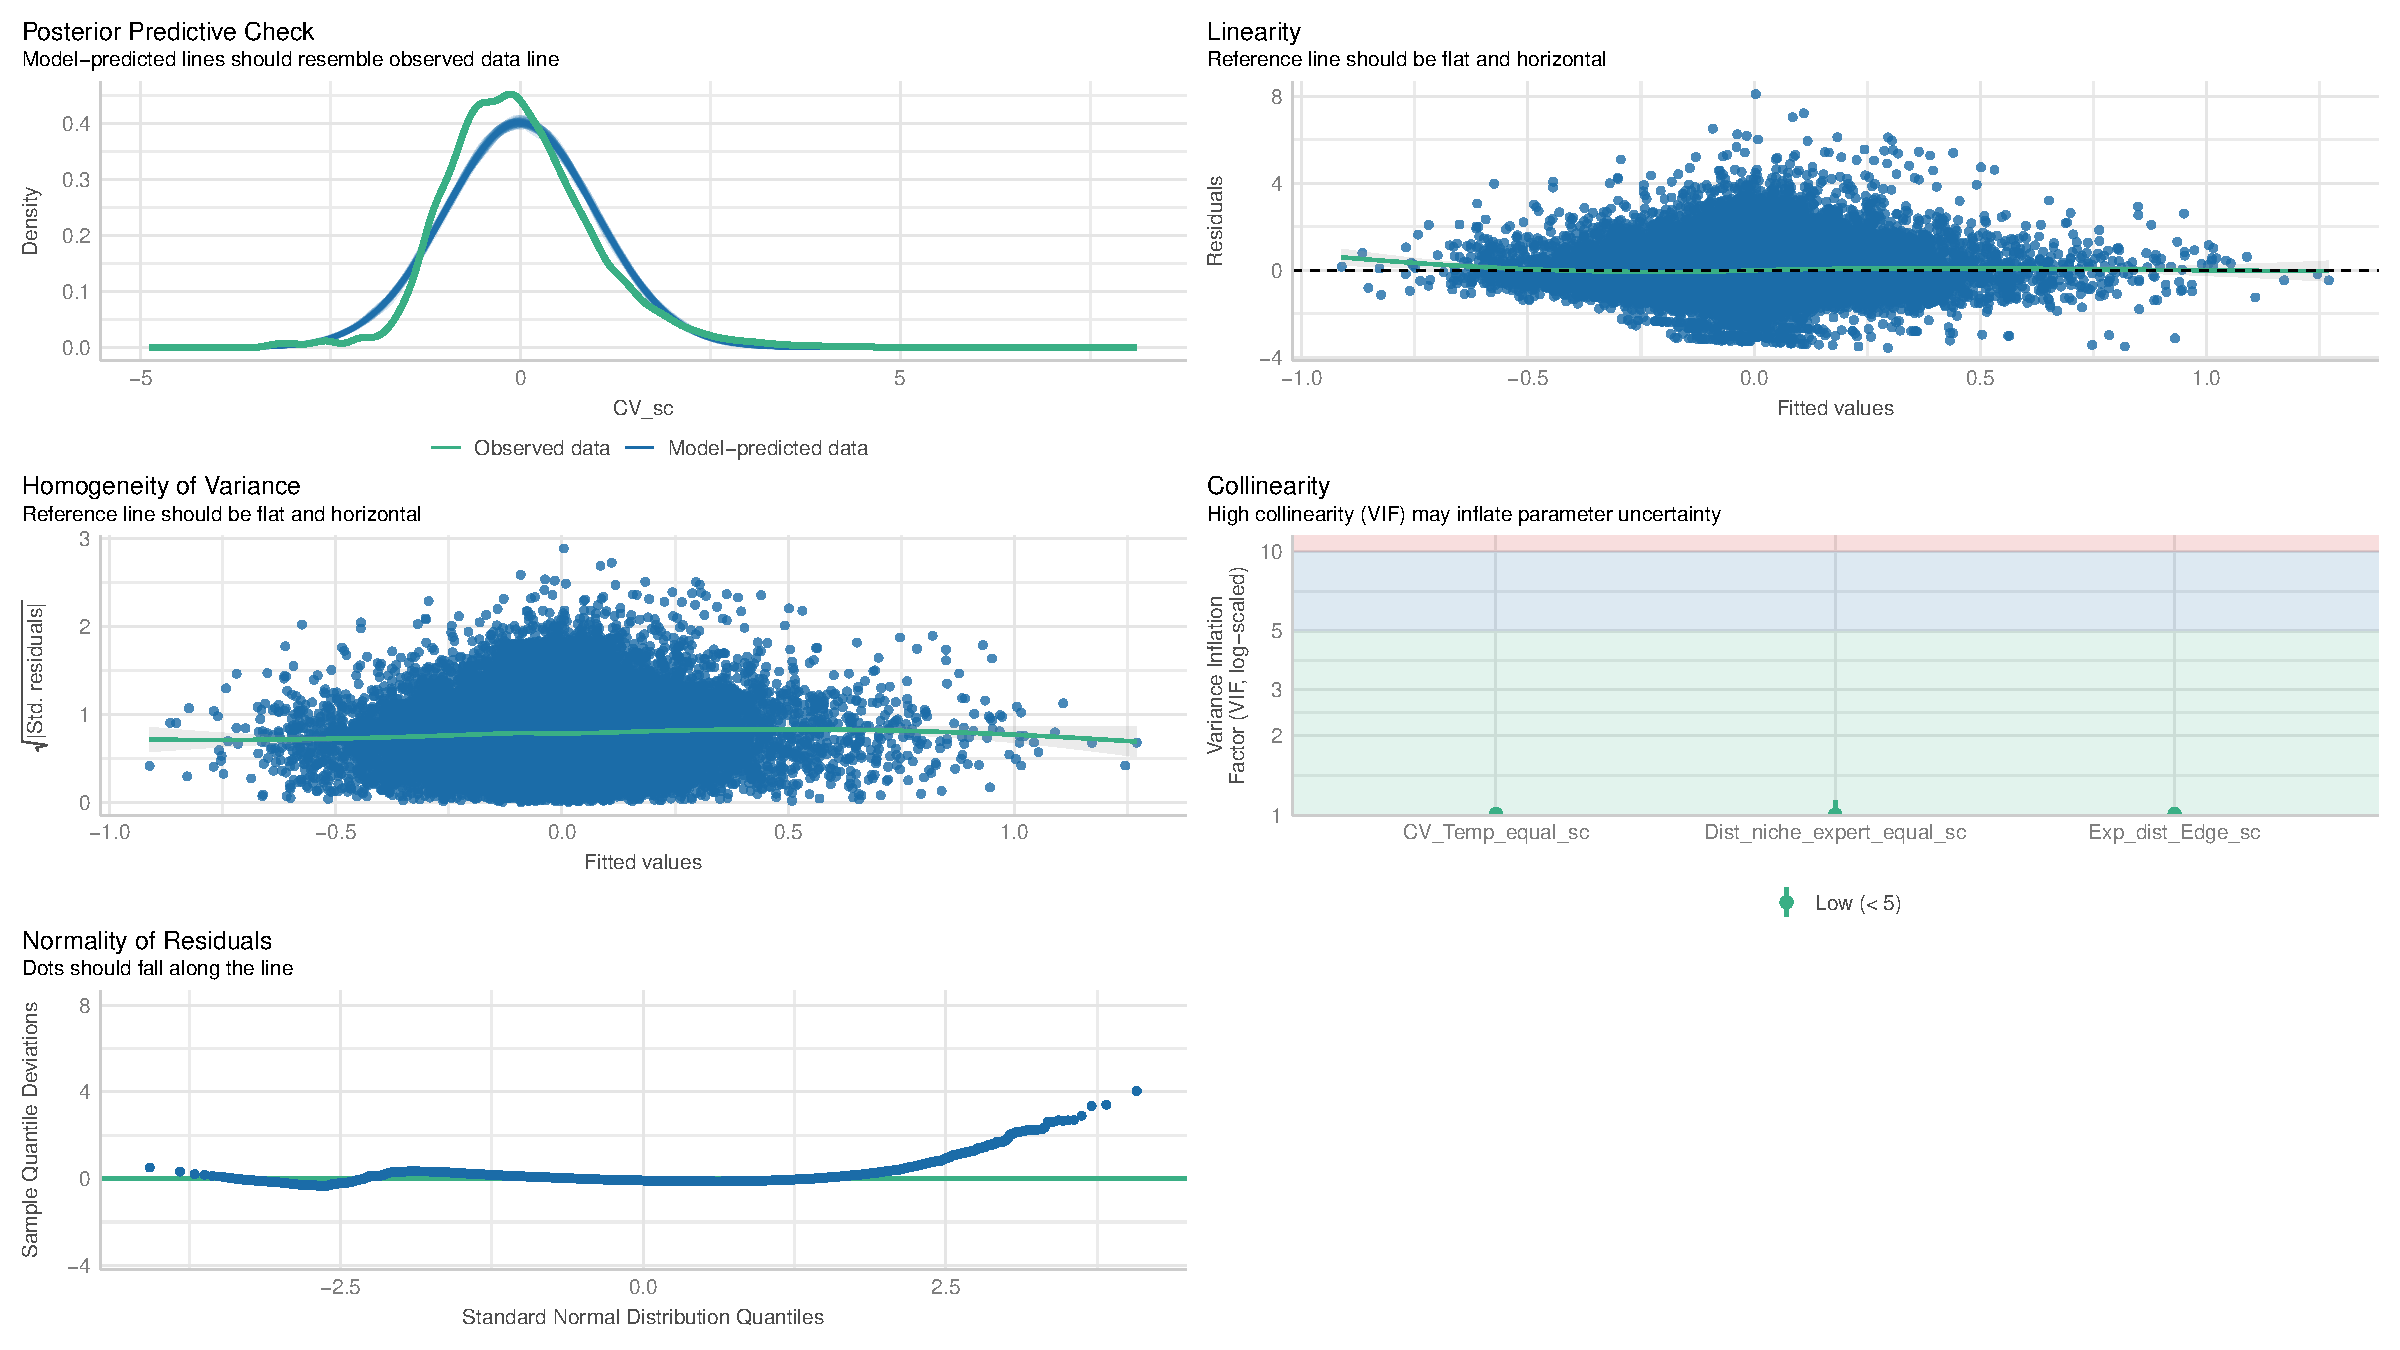
\includegraphics[width=1\textwidth]{FigRange/mod_edge}}
\caption[Edge model diagnostics]{Visual model diagnostics for the model that estimated distance to geographic range edges and climatic niche position from expert ranges, and that used temperature variability data aggregated from Behrmann equal area projection, as predictors (Table \ref{tab:lmm_edge}). Overall, the gaussian family fits well to the response variable that we used in the models (CV$\_$sc; scaled population variability), the linearity assumption is met, variance is homogeneous, and there is low correlation between the predictor variables (i.e., variance inflation factor (VIF) < 5), and the residuals are normally distributed.}  
\label{fig:edge_mod}
\end{figure}

\begin{figure}[H]
\centering
\centerline{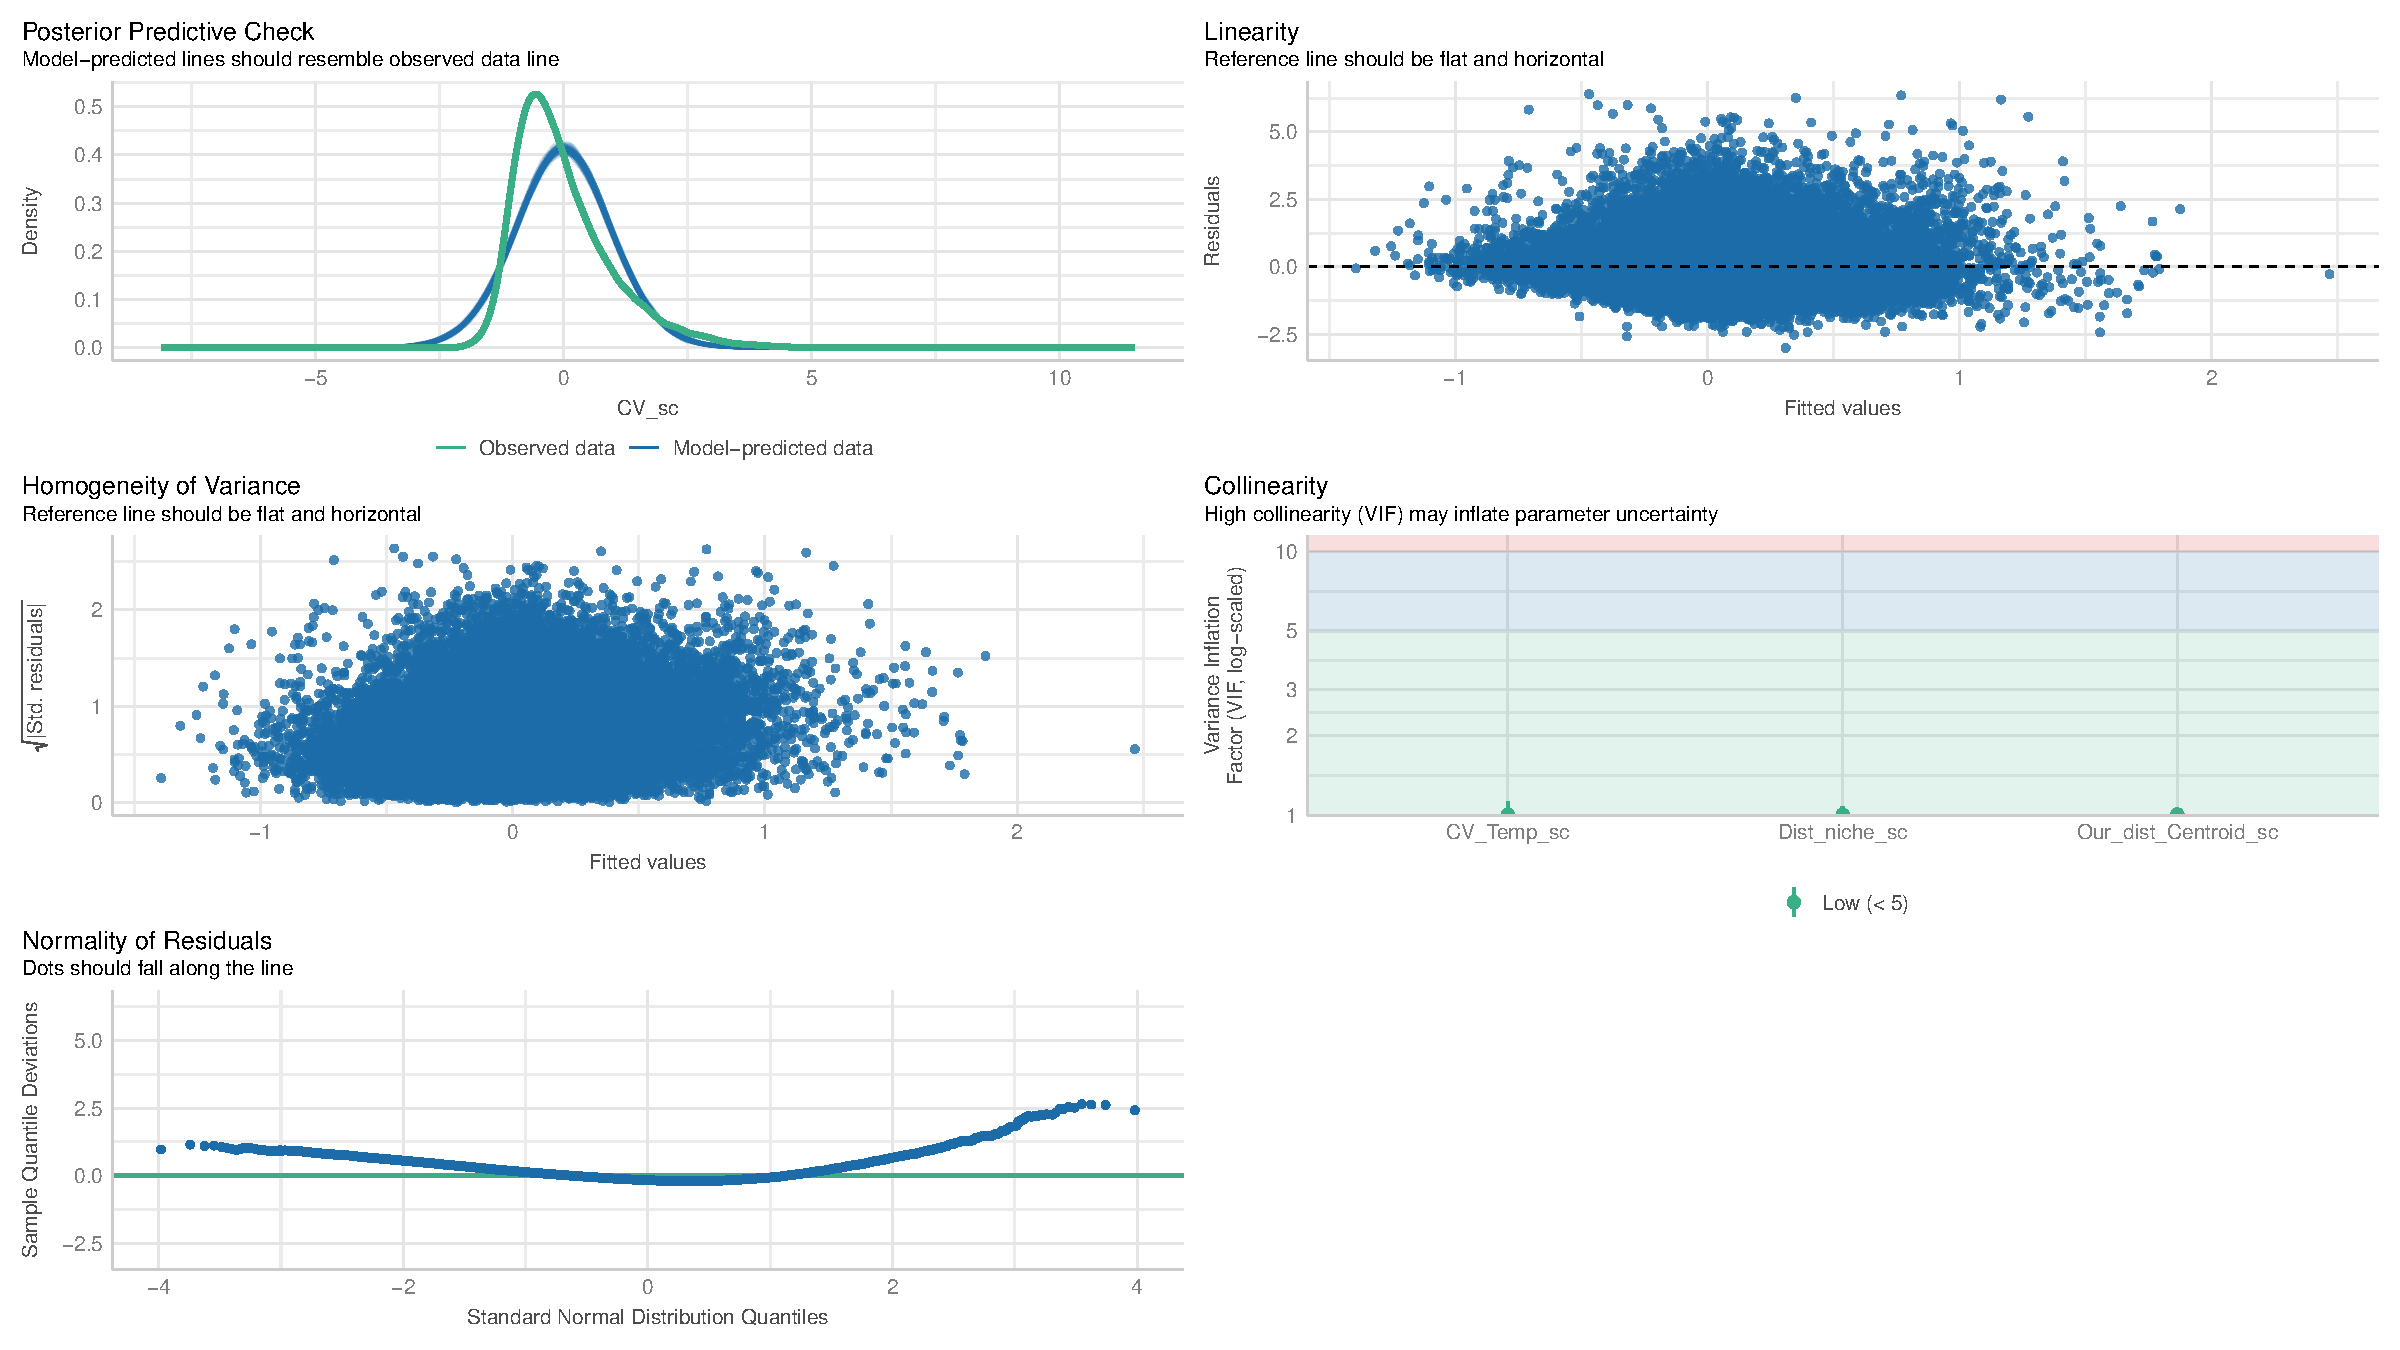
\includegraphics[width=1\textwidth]{FigRange/mod_0s}}
\caption[Zero model diagnostics]{Visual model diagnostics for the model where population variability was estimated considering zeros to years where a species was not recorded in a site, but that sampling event was done between the first and last year that a species was observed at a given site (Table \ref{tab:lmm_zeros}). Overall, the gaussian family fits well to the response variable that we used in the models (CV$\_$sc; scaled population variability), the linearity assumption is met, variance is homogeneous, and there is low correlation between the predictor variables (i.e., variance inflation factor (VIF) < 5), and the residuals are normally distributed.}  
\label{fig:0s_mod}
\end{figure}

\begin{figure}[H]
\centering
\centerline{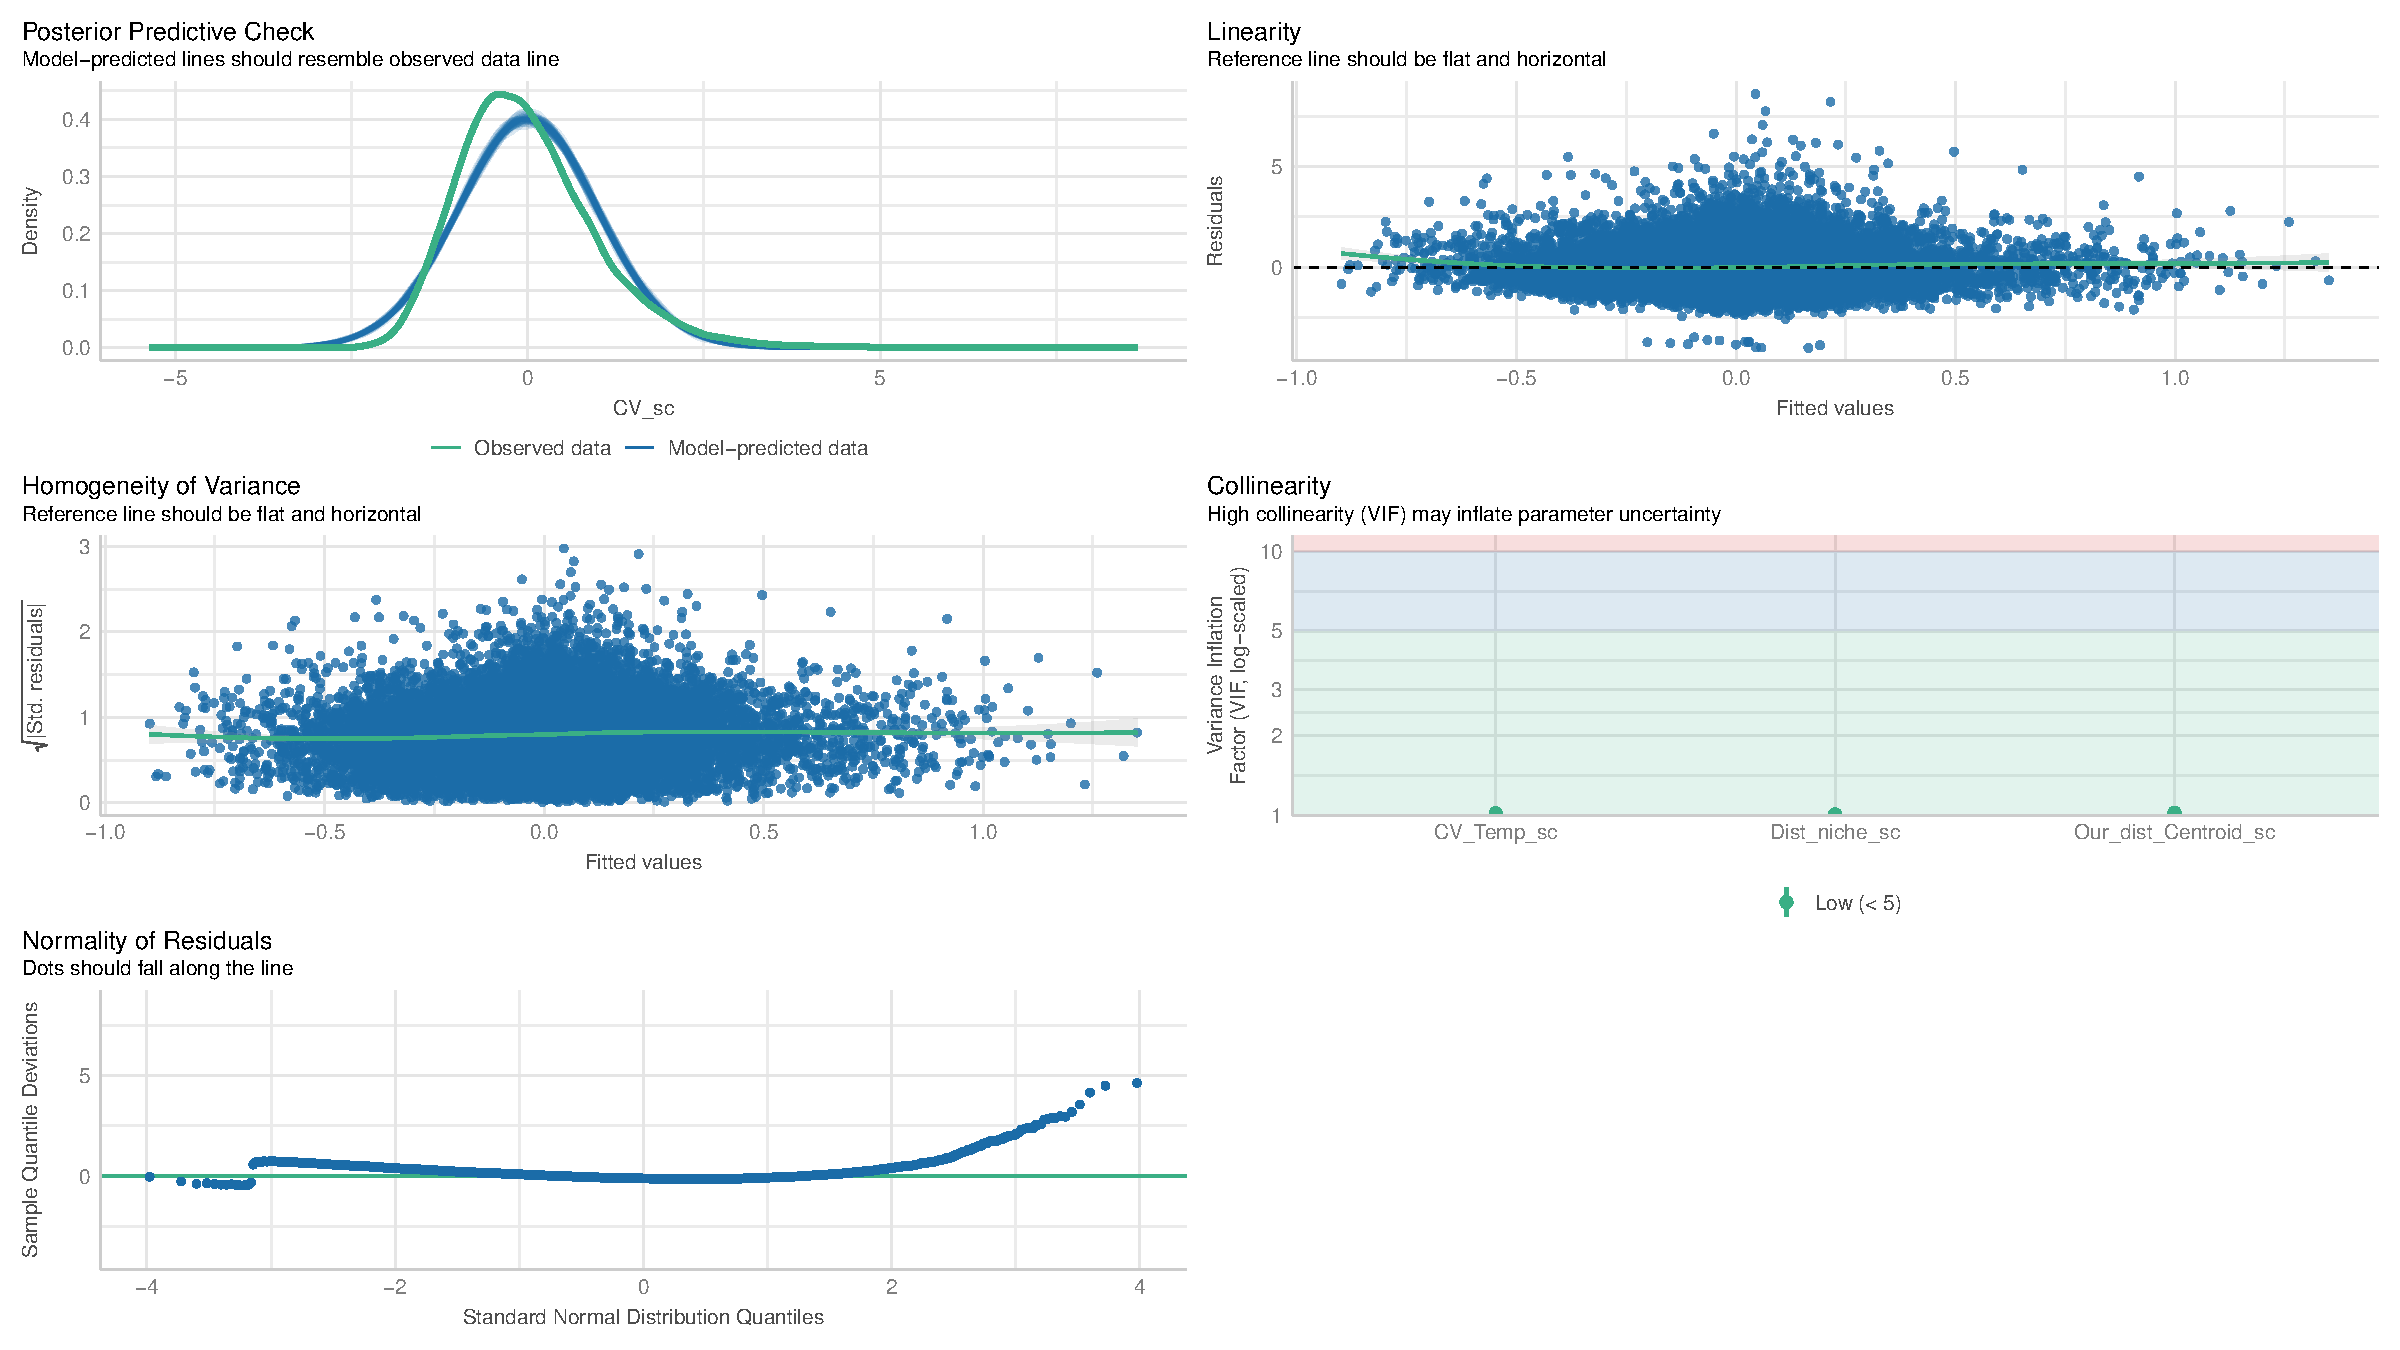
\includegraphics[width=1\textwidth]{FigRange/mod_10}}
\caption[Ten years model diagnostics]{Visual model diagnostics for the model where population variability was estimated considering only sites where species occupied for at least 10 years (Table \ref{tab:lmm_tens}). Overall, the gaussian family fits well to the response variable that we used in the models (CV$\_$sc; scaled population variability), the linearity assumption is met, variance is homogeneous, and there is low correlation between the predictor variables (i.e., variance inflation factor (VIF) < 5), and the residuals are normally distributed.}  
\label{fig:10_mod}
\end{figure}

\begin{figure}[H]
\centering
\centerline{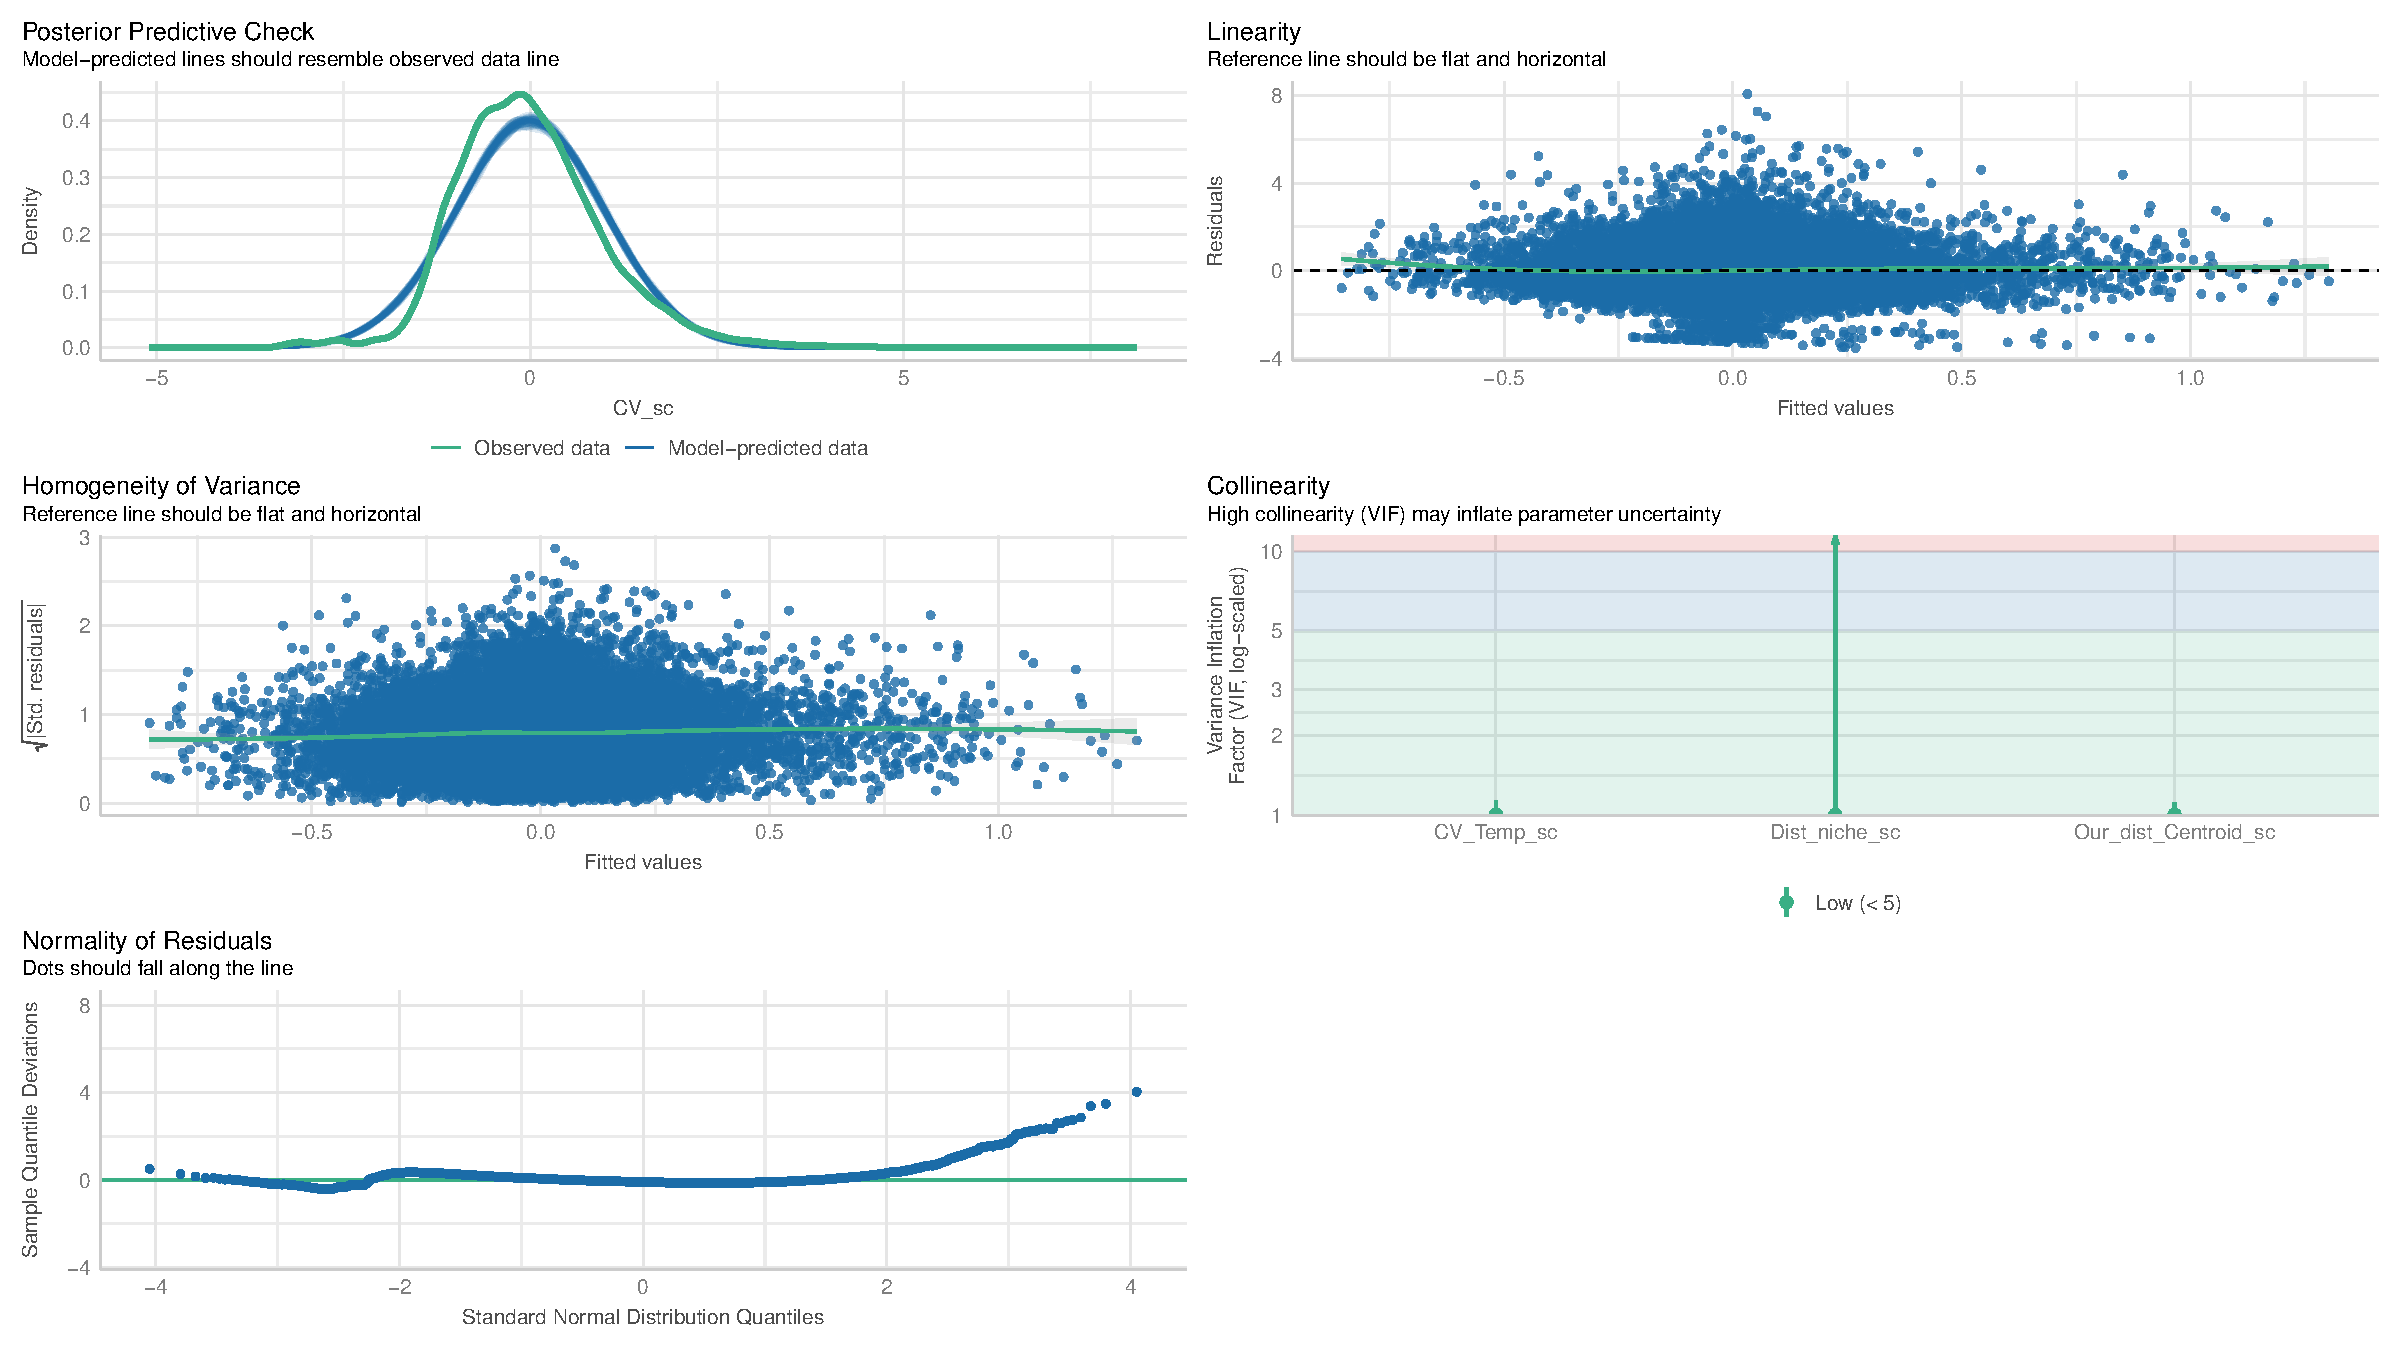
\includegraphics[width=1\textwidth]{FigRange/mod_comp}}
\caption[Range model diagnostics]{Visual model diagnostics for the model where we only considered the species that had $\geq$70\% of their geographic ranges sampled by BBS (Table \ref{tab:lmm_comp}). Overall, the gaussian family fits well to the response variable that we used in the models (CV$\_$sc; scaled population variability), the linearity assumption is met, variance is homogeneous, and there is relatively low correlation between the predictor variables (i.e., variance inflation factor (VIF) often < 5), and the residuals are normally distributed.}  
\label{fig:comp_mod}
\end{figure}

\section*{\textbf{Assessing the robustness of our results to methodological choices}}
Species geographic ranges and climatic niches can be estimated using different approaches that could affect our results. We used expert geographic ranges from birdLife and used these niches to estimate geographic range position and climatic niches. We estimated geographic range position as distance to range center and range edge. We did not estimate distance to geographic range edge for populations falling outside the expert ranges (i.e., these populations were removed from our analyses). The model fit using expert distance to range center considered 96 species (\textit{Aphelocoma woodhouseii} was removed from this analyses because it does not have expert ranges). Alternatively, the model fit using distance to range edge considered 94 species that had at least five populations sampled within their geographic ranges for five or more years. To estimate species climatic niches from expert ranges, we transformed these ranges and the bioclimatic variables (used to perform the PCA) to Behrmann equal area projection. All environmental values that fell within expert ranges were used to estimate species climatic niches. We also estimated temperature variability using Behrmann equal area to account for potentially different number of cells being aggregated across latitudes when estimating population variability for each route sampled by BBS. 
\paragraph*{}
Overall, we found the same results as reported in the main text regardless of how range position, climatic niches and temperature variability was estimated. Specifically, population variability was unrelated to distance to range center (Table \ref{tab:lmm_exp}) or range edge (Table \ref{tab:lmm_edge}) of expert geographic ranges. Population variability increased towards climatic niche limits when expert ranges were used to estimate climatic niches and in sites that had more variable temperatures when temperature was aggregated using equal area projection (Table \ref{tab:lmm_exp}).

% latex table generated in R 4.3.2 by xtable 1.8-4 package
% Wed Jan 22 10:41:08 2025
\begin{table}[ht]
\centering
\caption[Expert mixed effect model results]{Results from the linear mixed model that estimated distance to geographic range centers and climatic niches using expert ranges and temperature variability using Berhmann equal area projection. This model was fit considering 96 species. The results from this model are virtually the same as the results from the model presented in the main text, such that population variability increased towards climatic niche limits (Niche) and in variable temperatures (Temp.), but not near geographic range edges (Range). This model also had low explanatory power (conditional $R^2$ = 0.01). Bold p-values represent significant relationships. } 
  \vspace*{3mm}
\begin{tabular}{ccccc}
  \hline
 Predictor & Estimate & Std. Error & z value & Pr($>$|$z$|) \\ 
  \hline
  Intercept & 0.005 & 0.005 & 0.968 & 0.333 \\ 
  Niche & 0.039 & 0.013 & 2.946 & \textbf{0.003} \\ 
  Range & -0.002 & 0.015 & -0.151 & 0.880 \\ 
  Temp. & 0.037 & 0.014 & 2.688 & \textbf{0.007} \\ 
   \hline
\end{tabular}
\label{tab:lmm_exp}
\end{table}

% latex table generated in R 4.3.2 by xtable 1.8-4 package
% Wed Jan 22 10:53:33 2025
\begin{table}[H]
\centering
\caption[Edge mixed effect model results]{Results from the linear mixed model that estimated distance to geographic range edges and climatic niches using expert ranges and temperature variability using Berhmann equal area projection. This model was fit considering 94 species. The results from this model are virtually the same as the results from the model presented in the main text, such that population variability increased towards climatic niche limits (Niche) and in variable temperatures (Temp.), but not near geographic range edges (Range). This model also had low explanatory power (conditional $R^2$ = 0.01). Bold p-values represent significant relationships. } 
  \vspace*{3mm}
\begin{tabular}{ccccc}
  \hline
 Predictor & Estimate & Std. Error & z value & Pr($>$|$z$|) \\ 
  \hline
  Intercept & 0.004 & 0.005 & 0.768 & 0.442 \\ 
  Niche & 0.043 & 0.014 & 3.110 & \textbf{0.002} \\ 
  Range & 0.000 & 0.013 & 0.024 & 0.981 \\ 
  Temp. & 0.037 & 0.014 & 2.538 & \textbf{0.011} \\ 
   \hline
\end{tabular}
\label{tab:lmm_edge}
\end{table}

%%PASTE TABLES HERE?
\paragraph*{}
In the main text we estimated population variability considering only sites that a species was observed to occur for at least five years. In this case, species absences in sites between the first and last years that they were observed in a site (i.e., a density of zero) were not considered when estimating population variability. Here, we loosen this assumption and assigned a density of zero to sampling events where a species was not recorded in a site, but that sampling event was done between the first and last year that a species was recorded at a given site. Thus, a species observed during two years in a site could still be included in our analyses if that sites was sampled at least three times between the two observations (i.e., this species would have a density of zero for three years and a density > zero for the two years it was recorded). For this model, the 99 resident species were considered for our analyses as they had over five sites sampled for at least five years within their geographic ranges. In this case, we observed the same relationship as reported in the main text between population variability and climatic niche position and temperature variability. However, population variability also increases towards geographic range edges in this model (Table \ref{tab:lmm_zeros}).  This suggests that some sites are only temporally occupied by the species and that including zeros increases population variability in these sites (Figure \ref{fig:temp_occ}) such that patterns of population variability across geographic ranges become more evident in these cases.
%North American birds are shifting their geographic distributions due to recent climate change \citep{lasorte2007, zurell2024, martins2024} and may not have been able to successfully establish populations near range edges or may be more likely to experience local extirpations in these areas \citep{hampe2011,hargreaves2014,boakes2018, angert2020}
% In that case, years that were sampled and that a species  Here, we loosen 
%We also assessed whether the relationship between population variability and geographic range position, climatic niche position, and temperature variability is dependent on how population variability is estimated. 

We also estimated population variability using a more conservative estimate, where only sites species were observed to occur for at least 10 years were considered in the estimation of population variability. For this model, we considered 90 for our analyses that had over five sites sampled for at least five years within their geographic ranges. Similar to the main text results, population variability increased near niche limits and in variable temperatures. However, in this case we also observed that population variability increased towards geographic range edges (Table \ref{tab:lmm_tens}). This result suggests that time series length can be important to detect population variability patterns. Specifically, longer time series are more likely to capture higher variability in population densities that could be caused by different mechanisms. For example, long-term population trends may only be detected with longer time series, but longer time series may also be more likely to capture populations that are recovering from infrequent, but severe, disturbances that causes substantial changes in population densities over time. %This would explain the increase in population variability near range edges that we observed when considering populations that were recorded for at least 10 years in our analyses.

% latex table generated in R 4.3.2 by xtable 1.8-4 package
% Wed Jan 22 11:05:09 2025
\begin{table}[ht]
\centering
\caption[Zero mixed effect model results]{Results from the linear mixed model that assigned a density of zero to sampling events where a species was not recorded in a site to estimate population variability. This model was fit considering 99 species. In this case we observed that population variability increased towards climatic niche limits (Niche), geographic ranges edges (Range) and in variable temperatures (Temp.). This model also had low explanatory power (conditional $R^2$ = 0.05). Bold p-values represent significant relationships.} 
  \vspace*{3mm}
\begin{tabular}{ccccc}
  \hline
 & Estimate & Std. Error & z value & Pr($>$|$z$|) \\ 
  \hline
  Intercept & 0.005 & 0.005 & 1.036 & 0.300 \\ 
  Niche & 0.072 & 0.016 & 4.411 & \textbf{<0.001} \\ 
  Range & 0.063 & 0.017 & 3.640 & \textbf{<0.001} \\ 
  Temp. & 0.159 & 0.019 & 8.273 & \textbf{<0.001} \\ 
   \hline
\end{tabular}
\label{tab:lmm_zeros}
\end{table}


% latex table generated in R 4.3.2 by xtable 1.8-4 package
% Wed Jan 22 10:58:34 2025
\begin{table}[ht]
\centering
\caption[Ten years mixed effect model results]{Results from the linear mixed model that only considered sites where species were observed for 10 years to estimate population variability. This model was fit considering 90 species. In this case we observed that population variability increased towards climatic niche limits (Niche), geographic ranges edges (Range) and in variable temperatures (Temp.). This model also had low explanatory power (conditional $R^2$ = 0.02). Bold p-values represent significant relationships. } 
  \vspace*{3mm}
\begin{tabular}{ccccc}
  \hline
 Predictor & Estimate & Std. Error & z value & Pr($>$|$z$|) \\ 
  \hline
  Intercept & 0.025 & 0.007 & 3.876 & \textbf{<0.001} \\ 
  Niche & 0.078 & 0.015 & 5.044 & \textbf{<0.001} \\ 
  Range & 0.036 & 0.014 & 2.512 & \textbf{0.012} \\ 
  Temp. & 0.081 & 0.018 & 4.411 & \textbf{<0.001} \\ 
   \hline
\end{tabular}
\label{tab:lmm_tens}
\end{table}

\begin{figure}[H]
\centering
\centerline{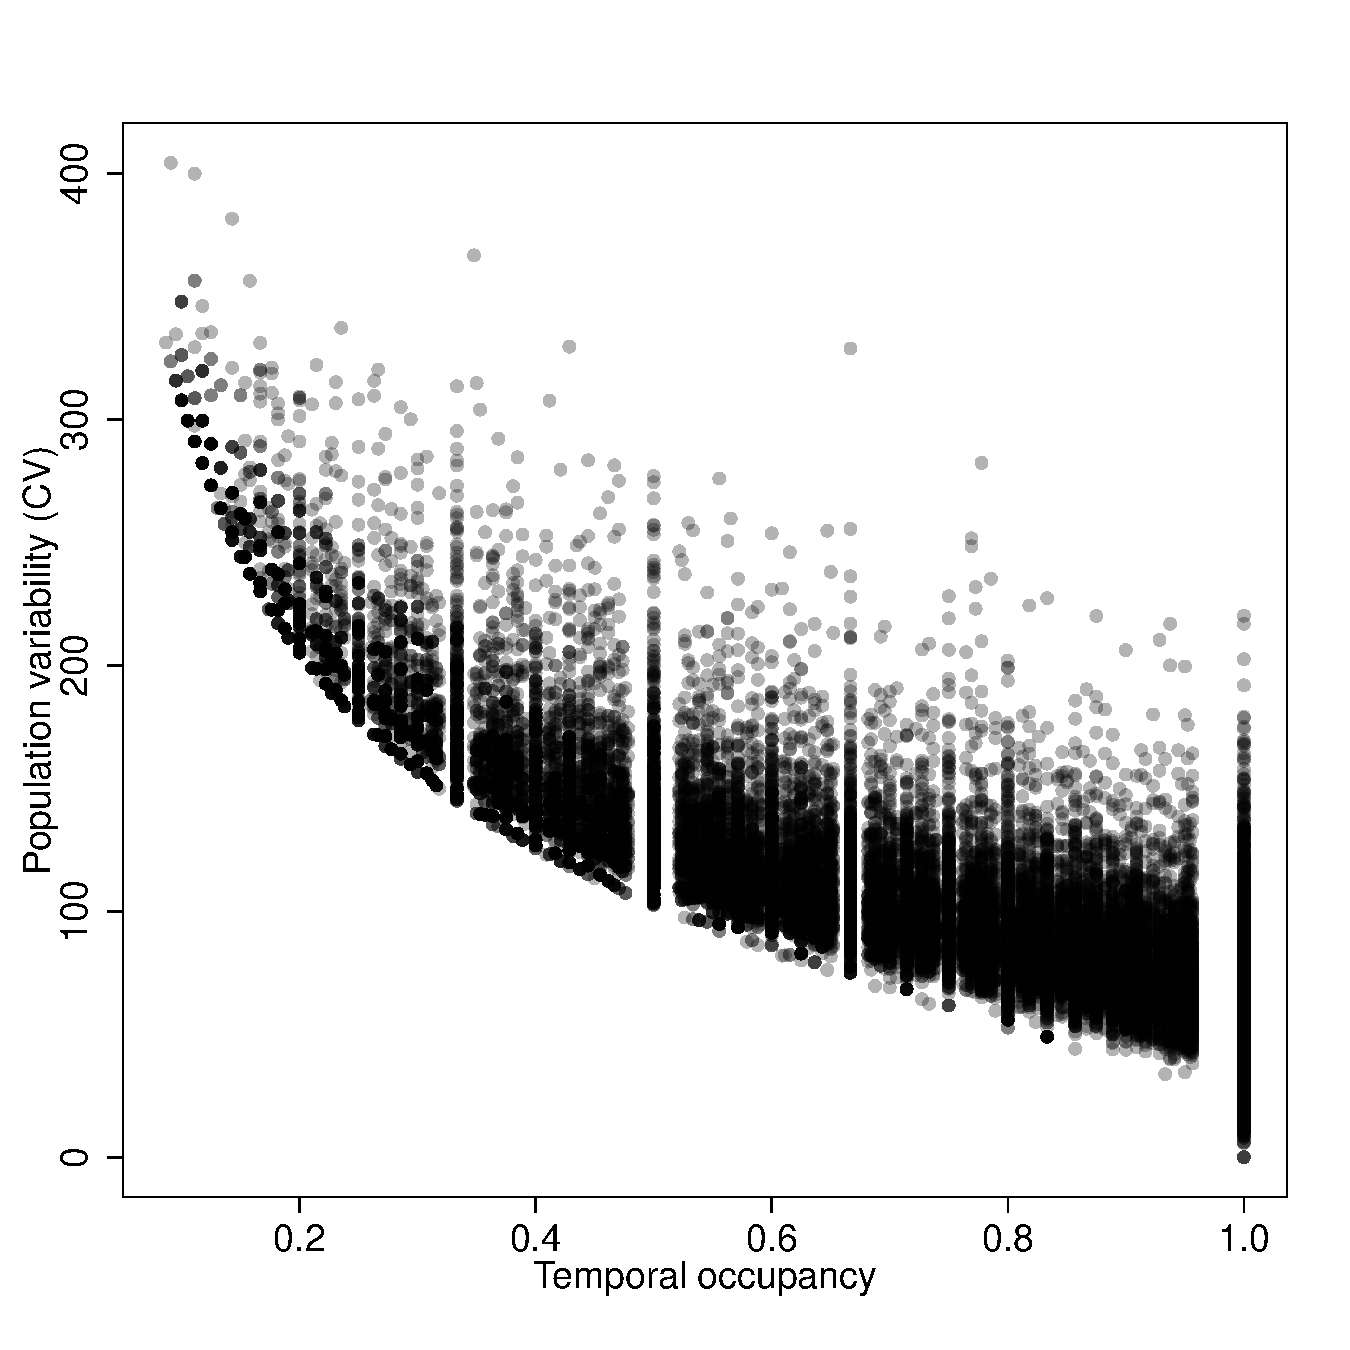
\includegraphics[width=1\textwidth]{FigRange/temp_occ}}
\caption[Temporal occupancy]{There is a strong relationship ($r$ = 0.90, $p < 0.001$) between population variability and population temporal occupancy in a site when zeros are considered during the estimation of population variability.}  
\label{fig:temp_occ}
\end{figure}

In the main text we evaluated the relationship between population variability and geographic range position, climatic niche position, and temperature variability using 97 resident bird species. Here, we restricted our analysis to consider only the species ($n = 52$) that had $\geq$70\% of their geographic ranges sampled by BBS to assess whether our results could have been affected by species that only have a small portion of their range sampled by BBS.  We found the same results as the ones reported in the main text, where popualtion variability increases towards climatic niche limits and in variable temperatures, but not near geographic range edges (Table{\ref{tab:lmm_comp}}. This indicates that considering resident species that have a small portion of their range sampled by BBS did not affect our results.


% latex table generated in R 4.3.2 by xtable 1.8-4 package
% Wed Jan 29 10:54:29 2025
\begin{table}[ht]
\centering
\caption[Range mixed effect model results]{Results from the linear mixed model that only considered species that had $\geq$70\% of their geographic ranges sampled by BBS. This model was fit considering 52 species. The results from this model are virtually the same as the results from the model presented in the main text, such that population variability increased towards climatic niche limits (Niche) and in variable temperatures (Temp.), but not near geographic range edges (Range). This model also had low explanatory power (conditional $R^2$ = 0.01). Bold p-values represent significant relationships.} 
\vspace*{3mm}
\begin{tabular}{ccccc}
  \hline
 & Estimate & Std. Error & z value & Pr($>$|$z$|) \\ 
  \hline
  Intercept & 0.010 & 0.006 & 1.681 & 0.093 \\ 
  Niche & 0.053 & 0.016 & 3.370 & \textbf{0.001} \\ 
  Range & 0.026 & 0.016 & 1.583 & 0.113 \\ 
  Temp. & 0.057 & 0.019 & 3.029 & \textbf{0.002} \\ 
   \hline
\end{tabular}
\label{tab:lmm_comp}
\end{table}
